% Innehållet i Vasungavisor 2010
%
% Kapitel "I Högan Nord"

\clearpage
\songchapter{Ur Törstiga Strupar}
\begin{figure}[!b]
\begin{center}

\includegraphics[width=5cm]{../bilder/fardigabilder/BilderTillKapitel/brannvin.png} 
\end{center}
\end{figure}
\clearpage
\begin{intersong}

\textbf{SNAPSARNAS NAMN}

\begin{small}
Alltsedan den blida tid då vårt brännvin uppfanns, har umgänget med detsamma varit omgärdat av en stängeligen upprätthållen ritual. Vad vi vet därom förtäljer traditionen. Brännvinet inmundigades i bestämda kvantiteter benämnda ''Snapsen'' eller ''Supen''. Enär dessa av goda skäl inte kunde tillåtas intagas godtyckligen, fick de snart alltefter sina rituella ordningsnummer specifika namn, av vilka vi idag känna tretton. Dessa är Helan, Halfvan, Tersen, Quarten, Quinten, Rifvan, Rafflan, Rännan, Smuttan, Smuttans unge, Femton droppar, Lilla Manasse och Lilla Manasses broder. Detta kulturarv bjuder oss att följa denna ritual och inte tillåta stundens nycker nagga dryckesdisciplinen i kanten. Vad skulle våra dryckesfäder känna i sina hjärtan om de från sina molnkanter nedblickade på en snapsritual innehållande ''Langbeinakrank'' istället för Rifvan och ''Tjorven'' eller, hemska tanke ''Sjunkbomben'' istället för den ärevördiga Lilla Manassen? Ruelse och vemod! Sentida studenter plägnar dock att utöver de traditionella alltefter tillfället tillägga snapsarna 
\end{small}
\end{intersong}

\begin{intersong}
\begin{small}
Kreaturets återuppståndelse och Inspektors klagan. Detta kunde emellertid klandras med avseende på måttlighet i denna värld befolkad av ett i fysisk måtto något förvekligat släkte, men som bekant tillhör inte omåttlighet dödssynderna, ej heller är måttlighet den högsta av dygder. Dock torde detta gruvligen utökade antalet snapsar anses vara ett förvekligat släkte tillfyllest. Efterföljande samling gör inte anspråk på uttömlighet ifråga om de olika smakriktningarna inom supvisornas genre, från tradition till vomeringsromantik, men likförbannat bör de uppstämmas med samma kraft som fordom innan snapsen under andaktsfull tystnad intagas. I kvistiga fall angående melodi eller dryckesdisciplin torde man vända sig till någon äldre vasung, lämpligen sångledaren (vasungen med sångvärjan; akta dig för den, du).
\end{small}
\end{intersong}
\clearpage
\input{Helan.tex}
\input{Halvan.tex}
\input{Tersen.tex}
\clearpage
\input{Kvarten.tex}
\beginsong{Magnus Öhmans kvint}[
	by={Hedersmedlem Magnus Öhman},					
	sr={Tryggare kan ingen vara}]					
	
\beginverse*
När man tagit fjärde supen
Känns det ännu strävt i strupen
Därför tar man lilla kvinten
Då blir strupen len som flinten!
\endverse									
\endsong							

\clearpage
\input{Halvankaren.tex}
\beginsong{Muminhalvan}[
	by={melodi Benny Törnroos},					
	sr={Muminvisan}]					
	
\beginverse*
När Helan är tagen
då väntar ju magen på Halvan!
För Helan togs först den,
men nu pockar törsten på Halvan!
Immig i glaset den kall mot oss ler,
Länge behöver vi ej vänta mer
på Halvan, på Halvan, på Halvan!
\endverse									
\endsong							

%\input{DenSallskapssjukaHalvan.tex}
\clearpage
\input{DetSattEnMas.tex}
\begin{figure}[!b]
\begin{center}
\includegraphics[width=25mm]{../bilder/mas.jpg} 
\end{center}
\end{figure}
\clearpage
\input{TillSupenTagerMan.tex}
\clearpage
\beginsong{Kräftinstruktioner}[ 		
	by={Isak Frants},		
	sr={Blinka lilla stjärna där}]										

	
\beginverse*						
Nu vi kräftor äta ska
hoppas att det smakar bra.
Röda, kokta, saltade
någon säger hatade.
Om man inte äta vill,
sjung då med och sitt snällt still. 
\endverse						

\beginverse				
Första steget är att då,
hål med kniv i ryggen få.
Saften sen man suger ut,
vips så har den tagit slut.
Borta utan något blink,
passar bra som god fördrink.
\endverse				

\beginverse				
Bryt sen båda klorna loss,
sug ur armarna förstås.
Klorna bändes upp så att, 
fram man får en liten skatt.
Köttbit upplagt som på spätt,
ger oss munsbit till förrätt.
\endverse				

\beginverse				
Vrid sen modigt stjärten väck,
alltså kräftans lilla häck. 
Skala allt som int' är mjukt,
vassa kanter kan ta sjukt.
Se det gick ju riktigt lätt,
grattis här din huvudrätt.
\endverse				

\beginverse				
Sist ut då men inte minst,
kräftans egna gyllna vinst.
Likt en hög av guldpengar,
ligger kräftsmör nu schennar. 
Kniv i hand och svep det slätt,
svårt att slå sån efterrätt.
\endverse				
\endsong	

\clearpage
\beginsong{Imbelupet}[ 							
	sr={Kors på Idas grav}]		
	
\beginverse*						
Imbelupet glaset står på bräcklig fot,
kalla pilsnerflaskor luta sig därmot,
men därnere, miserere, uti magens avgrundsdjup,
sitter djävulen och väntar på en sup.
\endverse						

\beginverse				
Imbelupet glaset står på bräcklig fot,
kalla pilsnerpavor luta sig därmot,
men därnere, miserere, uti magens dunkla valv,
vankar djävulen i väntan på en halv.
\endverse				

\beginverse				
Imbelupet glaset står på bräcklig fot,
importerad bajerskt luta sig därmot,
men därnere, miserere, uti magen härs och tvärs,
knallar djävulen och väntar på en ters.
\endverse				

\beginverse				
Imbelupet glaset står på bräcklig fot,
klena lättölspavor luta sig därmot,
men därnere, miserere, uti magen djup och svart,
rusar djävulen och väntar på en kvart.
\endverse				

\beginverse				
Imbelupet glaset står på bräcklig fot,
ljumma starkölsflaskor luta sig därmot,
men därnere, miserere, uti magens labyrint,
irrar djävulen i väntan på en kvint.
\endverse				

\beginverse				
Imbelupet glaset står på bräcklig fot,
glömda folkölsburkar luta sig därmot,
men därnere, miserere, uti magens slingerväxt,
sitter själve fan och väntar på en sext.
\endverse				

\beginverse				
Imbelupet glaset står på bräcklig fot,
kalla pilsnerhalvor luta sig därmot,
men därnere, miserere, sitter allas våran far
det är fan och han vill ha det som är kvar!
\endverse				
\endsong	

\clearpage
\beginsong{Här kommer spriten!}[ 							
	sr={Text: Matias Strandberg och Anna Jutila, melodi: "I mumindalen"}]		
	
\beginverse*						
Vem kommer glatt till festen här?
Jovisst, det törstig gulis är!
Med raska steg och noll balans
Önskar sig att dricka fanns
\endverse						

\beginverse				
Här kommer spriten! 
Här kommer spriten!
\endverse				

\beginverse				
Här kommer spriten! x4
\endverse				

\beginverse				
Refräng x2
Öl-öl-öl-öl
Öl-öl
Öl-öl-bisse!
\endverse				

\beginverse				
Lo-lo-lo-lo
Lo-lo
Lo-lo-lonkku!
\endverse				

\beginverse				
Öl-öl-öl-öl-öl
Cider och lonkero!
\endverse				
\endsong	

\clearpage
\beginsong{Gå på fest}[ 							
	sr={Du ska få min gamla cykel},					
	index={När som livet kännes},
	index={Är du vissen}]		
	
\beginverse*						
När som livet kännes mörkt och grått och trist,
GÅ PÅ FEST
När humöret allt emedan du mist,
GÅ PÅ FEST
När du tror att allting grånar, 
ska du se att himlen blånar, 
sommarns blommor dig förvånar, 
GÅ PÅ FEST!
\endverse						

\beginverse				
Är du vissen, klen och trött och matt och svag, 
GÅ PÅ FEST
Skulle hjärtat bara slå vartannat slag, 
GÅ PÅ FEST
Strunt i doktorn och recepter, 
medicin och farmacepter, 
sluta upp och känna efter, 
GÅ PÅ FEST!
\endverse				
\endsong
\clearpage
\beginsong{Härjarvisan}[ 	
    by={Hasse Alfredsson},						
	sr={Gärdebylåten},					
	index={Nu ska vi ut och härja}]		

\beginverse*
Liksom våra fäder vikingarna i Norden,
drar vi landet runt och super oss under borden.
Brännvinet har blitt ett elexir 
för kropp såväl som själ.
Känner du dig liten och ynklig på jorden,
växer du med supen och blir stor uti orden.
Slår dig för ditt håriga bröst,
och blir en man från hår till häl.
\endverse

\beginchorus				
Ja, nu skall vi ut och härja,
supa och slåss och svärja,
bränna röda stugor, slå små barn
och säga fula ord!
Med blod skall vi stäppen färga.
Nu änteligen lär jag
kunna dra nån riktig nytta av
min Hermodskurs i mord! 
\endchorus	

\beginverse					
Hurra, nu skall man änteligen få röra på benen,
hela stammen jublar och det spritter i grenen.
Tänk att än en gång få spränga fram
på Brunte i galopp!
Din doft, o kära Brunte är trots brist i hygienen,
för en vild mongol minst lika ljuv som syrenen.
Tänk att på din rygg få rida runt
i stan och spela topp. 
\endverse						

\beginchorus				
Ja, nu skall vi ut och härja ...
\endchorus	

\beginverse
Ja, mordbänder är klämmiga, ta fram fotogenen!
Och eftersläckningen tillhör just de fenomenen
inom brandmansyrket, som jag tycker 
det är nån nytta med.
Jag målar för mitt inre upp den härliga scenen: 
blodrött mitt i brandgult. Ej ens prins Eugen en
lika mustig vy kunnat måla, 
ens om han målade med sked. 
\endverse	

\beginchorus	
Ja, nu skall vi ut och härja ... 
\endchorus	
\endsong

\input{FordomOdladeMan.tex}
%\clearpage
%\beginsong{Heppeneppetepp}[ 						
	index={Till Stockholm for}]		
	
\beginverse*						
Till Stockholm for Heppeneppetepp, 
till Stockholm for jag.
Till Stockholm for Heppeneppetepp,
till Stockholm for jag.
\endverse	
\beginchorus
/: Till Stockholm for Amalia
som bad oss supa bra, 
och till Stockholm for alla raska gossar
som i laget där var.:/
\endchorus		

\beginverse				
Och supen tog Heppeneppetepp
och supen tog jag.
Och supen tog Heppeneppetepp
och supen tog jag.
\endverse	
\beginchorus
/: Och supen tog Amalia...:/
\endchorus	

\beginverse
I finkan kom Heppeneppetepp
i finkan kom jag. 
I finkan kom Heppeneppetepp
i finkan kom jag.
\endverse	
\beginchorus
/: I finkan kom Amalia...:/
\endchorus

\beginverse
Men frikänd blev Heppeneppetepp
och frikänd blev jag. 
Men frikänd blev Heppeneppetepp
och frikänd blev jag. 
\endverse	
\beginchorus
/: Och frikänd blev Amalia...:/
\endchorus	
\endsong		

\clearpage
\input{HurLangeSkallPaBordet.tex}
\beginsong{Det perfekta glaset}[
	by={Nicklas Forss},
	sr={Sommardag i Kangasala},
	index={Jag lyfte den lilla supen}]
	
\beginverse*						
Jag lyfte den lilla supen
och hällde den i min hals.
Det kittla så härligt i strupen,
men kvar fanns sen inget alls.
Jag titta på glaset och drömde
att det hade sådan funktion:
/: hur mycket man än ur det tömde,
där alltid fanns kvar en portion.:/
\endverse						
\endsong		

\clearpage
\input{KassenFull.tex}
\beginsong{Infinitesimal""differensen}[ 							
	sr={Hipp-hurra för Bamsefar},					
	index={Enligt Darwins teori}]		
	
\beginverse*						
Enligt Darwins teori
dag för dag utvecklas vi.
Men varför har vi högre rang
än Zoos orangutang?
\endverse						

\beginchorus
Jo, djuret vid sitt vattenhål
ser till vätskebalansen
och endast primitiva vrål
kan höras från seansen.
Men människan, ett högre djur,
tar glaset med förtjusning.
Hon sjunger uti moll och dur,
och dricker för berusning.
\endchorus

\beginverse				
Tänk på enda skillnaden,
så du respekterar den!
Tag dig därför ingen tår
om du ej kan ``Helan går''!
\endverse				
\endsong		

\clearpage
% Exempel på färdig-formaterad sång till VN:s
% sångbok 2018.

% Denna fil kan användas som sådan, bara verserna,
% namnen och annan rådata behöver bytas ur fälten.
% Tecknet "%" markerar en kommentar som helt och 
% hållet ignoreras av programmet som läser filen.

% Spara den färdiga filen som 
% 'SangnamnUtanMellanslagEllerSkander.tex'
% t.ex. blir "Vid En Källa" till 
% 'VidEnKalla.tex'
% Varje sång blir en egen fil.

\beginsong{Jag har aldrig vart på snusen}[ 	% Börja sången här
	by={},	% Författare
	sr={O hur saligt att få vandra}]		% Alternativa
			% sångnamn
	
\beginverse*		% Börja vers
Jag har aldrig vart på snusen,
aldrig rökat en cigarr - halleluja!
Mina dygder äro tusen,
inga syndiga laster jag har.
\endverse
\beginverse*
Jag har aldrig sett nå't naket,
inte ens ett litet nyfött barn.
Mina blickar går mot taket,
därmed undgår jag frestarens garn.
\endverse			% Sluta vers

\beginchorus
Halleluja, halleluja, 
halleluja, halleluja
halleluja, halleluja,
Hallelujaaa-aaa-a!
\endchorus

\beginverse*		% Börja vers
Bachus spelar på gitarren,
Satan spelar på sitt handklaver.
Alla djävlar dansar tango,
säg vad kan man väl önska sig mer?
\endverse
\beginverse*
Jo, att alla bäckar vore brännvin,
stadsparksdammen full av bayerskt öl,
konjak i varenda rännsten
och punsch i varendaste pöl.
\endverse			% Sluta vers

\beginchorus
Halleluja, halleluja...
\endchorus
\endsong			% Sluta sång

\clearpage
\input{Kosmonauten.tex}
\begin{figure}[!t]
\begin{center}
\includegraphics[width=6cm]{../bilder/kosmonauten.png} 
\end{center}
\end{figure}
\vspace{25mm}
\beginsong{Livet är härligt}[ 							
	sr={Pråmdragarna på Volga},
	index={Ta dig en vodka}]		
	
\beginverse*						
Livet är härligt,
tavaritj, vårt liv är härligt!
Vi alla våra små bekymmer glömmer, 
när vi har fått en tår på tand; en skål!,
\endverse						

\beginverse				
Ta dig en vodka, 
tavaritj, en liten vodka! 
Glasen i botten vi tillsammans tömmer,
det kommer mera efter hand; en skål!
\endverse

\textnote{Sången sponsoreras av Vasa nations inspektor 2015- Ilse Julkunen.}
\endsong		

\begin{figure}[!b]
\begin{center}
\includegraphics[width=6cm]{../bilder/livet_ar_harligt.jpg} 
\end{center}
\end{figure}
\clearpage
\beginsong{Mera brännvin}[ 						
	sr={Internationalen},					
	index={Internationalen}]		
	
\beginverse*						
Mera brännvin i glasen,
mera glas på vårt bord,
mera bord på kalasen,
mer kalas på vår jord.
\endverse						

\beginverse				
Mera jordar kring månen,
mera månar kring Mars,
mera marscher till Skåne,
mera Skåne - bevars!
\endverse			

\beginverse*						
Lisää viinaa mun lasiin,
lisää laseja pöydälle,
lisää pöytiä näihin juhliin,
lisää juhlia kansalle.
\endverse					

\beginverse				
Lisää kansaa Suomeen,
lisää Suomea päälle maan,
lisää maata Suur-Suomelle,
marssitaan, marssitaan, Karjalaan, Karjalaan! 
\endverse					

\vspace{1cm}	
\endsong		

\beginsong{Om cykling}[ 		
	by={Povel Ramel},					
	sr={Så väva vi vallman},					
	index={Man cyklar för litet}]		
	
\beginverse*						
Man cyklar för litet, 
Man röker för mycket.
Och man är fasen så liberal 
när det gäller maten och spriten. 
Man borde slutat för länge sedan
men denna sup är för liten. 
\endverse										

\beginverse*						
Vad tjänar att hyckla? 
Tids nog får man cykla! 
\endverse										

\endsong		

\clearpage
\beginsong{Minnet}[ 		
	by={T. Perret},					
	sr={Memories}]		
	
\beginverse*						
Minne! 
Jag har tappat mitt minne! 
Är jag svensk eller finne? 
Kommer inte ihåg.
Inne!
Är jag ut eller inne? 
Jag har luckor i minne, 
sån' där små alkohål. 
Men besinn' er, 
man tätar med det brännvin man får, 
när som minnet och helan går. 
\endverse						

\beginverse			
 Minne? Muisti hävis, mutt' minne?
Juhlista selvisimme
- muistikatkoja on.
Minne, lähtisin vaikka minne,
kunhan selvittäisimme
mitä tapahtunut on.
Mutta tiedän
mä keinon mikä auttaapi tuo:
Ota ryyppy, ja muistis juo!
\endverse				
\endsong		

\clearpage
\beginsong{Presidentvisan}[ 							
	sr={Och jungfrun hon går i ringen},					
	index={Och Mauno han satt på Gullranda}]		
	
\beginverse*						
Och Mauno han satt på Gullranda,
hojta på frun.
Men frun satt i andra ändan
ut i sin paulun.
Det eka' i valven som vette mot norr,
när Mauno gick till skåpet
för att ta sig en knorr.
\endverse						

\beginverse				
``Kom hit, ska vi ta en tuting,
fru Tellervo!''
Men Tellervo skrek tillbaka:
``Nej, Mauno, nå, nå!''
Men avståndet gör att man kan vara viss,
att Mauno han svälja och säga:``KIPPIS!''
\endverse				
\endsong		

\begin{figure}[!b]
\begin{center}
\includegraphics[width=30mm]{../bilder/hallandeflaska.jpg} 
\end{center}
\end{figure}
\clearpage
\beginsong{Rattataa}[
	index={Att dricka brännvin}]		
	
\beginverse*						
Att dricka brännvin är en sed
som ingen har oss lärt.
Från början vi ej kunde 
men det var blott temporärt.
Vi lärde oss så småningom
det var nog värt besvärt.
Tittilurenbom, tutidalenpang,
det var nog värt besvärt.
\endverse						

\beginchorus				
/: Rattataa, så tar vi oss en tuting,
rattataa, med mycket brännvin i.
Rattataa, rattataa
dricka brännvin gillar ja'
för jag blir så full och gla’.:/
\endchorus				
\endsong		

\clearpage
\beginsong{Brännvin, vatten}[ 	
	by={Atte och Jocke Boström},					
	index={Viinaa, vettä}]		
	
\beginverse*						
Brännvin, vatten,
 smakar skit som katten. 
Brännvin, helt rått,
:/ smakar jävligt gott!:/
\endverse
						
\beginverse				
Viinaa, vettä 
- mitä perkelettä? 
Viinaa raakaa 
/: napaan kaatakaa!:/
\endverse			

\vspace{1cm}	
\endsong		

%\clearpage
%\input{RenHelanSlunkitNer.tex}
\begin{figure}[!b]
\begin{center}
\includegraphics[width=5cm]{../bilder/skalandehander.jpg} 
\end{center}
\end{figure}
\clearpage
\beginsong{Rullaati, rullaati}[ 						
	index={Nu temperaturen är hög uti kroppen}]		
	
\beginverse*						
Nu temperaturen är hög uti kroppen, 
närmare 40 än 37.
 Men så skall det vara när ångan är oppe, 
och så är fallet uti detta nu. 
\endverse

\beginchorus				
Hej, rullaati rullaati rullaati rulla,
rullaati rullaati rullallalei! 
Hej, rullaati rullaati rullaati rulla,
rullaati rullaati rullallalei! 
\endchorus

\beginverse
Livet är kort som en barnunges tröja, 
ingenting kan vi väl göra åt det.
Men med vår sång kan bekymren vi röja, 
bort ifrån vardagens grådaskighet. 
\endverse	

\beginchorus
Hej rullaati...	
\endchorus

\beginverse
Snabbt flyktar ungdomens korta sekunder, 
skynda dig därför och räck mig din hand! 
Ej skall förgäves vi leva de stunder, 
då vi med sång knyter vänskapens band. 
\endverse	

\beginchorus
Hej rullaati...
\endchorus	
\endsong	

\begin{intersong}
	\begin{center}
		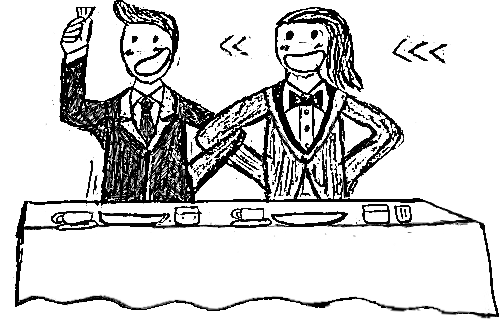
\includegraphics[width=0.6\textwidth]{../bilder/fardigabilder/CamillasFardigaBilder/Punschenkommer2.png} 
	\end{center}
\end{intersong}	
\clearpage
\beginsong{Gäddan och spriten}[ 							
	sr={Stenka Rasin},					
	index={Uppå väggen går en gädda}{Vodka, vodka}]		
	
\beginverse*						
Uppå väggen går en gädda, 
med långa ludna svarta ben.
:,: Men ni ska inte vara rädda,
ta en sup, och allt går väl! :,:
\endverse						

\beginverse				
Vita möss som gå i taket, 
råma hest och falla ner.
:,: Men ni ska inte vara rädda,
ta en sup, och allt går väl! :,:
\endverse
				
\beginverse				
Vodka, vodka vill jag dricka
jag vill äta kaviar.
:,: Jag vill älska russki flicka/pojke, 
jag vill spy i samovar :,:
\endverse	

\beginverse				
Koskenkorva vill jag dricka,
jag vill gå på kräftkalas.
:,: Jag vill älska Suomi-neito, 
jag vill spy i Aaltovas :,:
\endverse	
\endsong	

\clearpage
\input{Sibbovisan.tex}
\clearpage
\beginsong{Lemsjöholmsvisan}[
	by={melodi Väva vadmal, text: Gustac Elfving på Lemsjöholm sommaren 1976},					
	sr={Vitsvansade hjortar}]					
	
\beginverse*
Vitsvansade hjortar
Vitsvansade hjortar
Jag tror jag snapsar 
tills jag kollapsar
Vitsvansade hjortar.
\endverse									
\endsong							

\clearpage
\beginsong{Sörnai gusha}[ 										
	index={Oon vain köyhä poika}]		
	
\beginverse*						
Sörnai gusha nietu Molotova
sörnai gusha herba Moskova.
/: Njet, njet bonimai votvot risubuska,
dara zeva votvot harasoo.:/
\endverse

\beginverse				
Isa Stalin, äiti Hrustseva,
iski silmää ginihibragas.
/: Oi-oi oisiba vodkaa ollut heillä,
oisi isgu gäynyt alemmas.:/
\endverse

\beginverse
Tuoksuu tuomet, syreenit ja ruusut, 
tuoksuu tuolla Volgan randamill'.
/: Ai, ai kaunis kulta Kaditzuska,
tuoksuu tundeet rindas rindamill.:/
\endverse

\beginverse
Siellä missä versoaapi viljaa, 
siellä kasvoi kaunis Katjuska.
/: Katjuskalla komiat on keuhkot,
baska haisee Nevan rannalla.:/
\endverse

\beginverse
Siperian lakeus on suuri,
siellä Sonja lunta lapioi.
/: Sonjalla kävi hiton huono tuuri,
kun länsituuli uutta lunta toi. :,;
\endverse

\beginverse
Oon vain köyhä kolhoosinainen,
ei oo mulla yhtään ystävää.
/: Ei oo lehmää eikä ole lammasta,
eikä suussa yhtään hammasta.:/
\endverse

\beginverse
Oon vain köyhä poika Petroskoista,
ei oo mulla yhtään ystävää. 
/: Sirppi ja vasara ne taivahalla loistaa,
basga haisee, balalaikka soi.:/
\endverse		
\endsong		

\clearpage
\input{StruntISorger.tex}
\beginsong{Tänään otetaan}[ 						
	sr={Joulu on taas},
	index={Idag ska vi ha}]		
	
\beginverse*						
/: Tänään otetaan, tänään otetaan, 
helvetin paljon viinaa.:/
/: Huomenna on, huomenna on,
helvetin kova krapula.:/
\endverse						

\beginverse				
/: Idag ska vi ha, idag ska vi ha,
helvetes mycket brännvin.:/
/: Imorgon ska vi ha, imorgon ska vi ha,
helvetin kova krapula.:/
\endverse
		

\beginverse				
/: Täna võtame, täna võtame,
kuradima palju viina.:/
/: Homme meil on, homme meil on,
kuradima kova pohmakas.:/

\endverse			
\endsong		

\clearpage

\beginsong{Tänk om jag hade lilla nubben}[ 					
	sr={Hej tomtegubbar}]	
	
\beginverse*						
/:Tänk om jag hade lilla nubben
på ett snöre i halsen. :/
Jag skulle dra den upp och ner,
så att den kändes som många fler.
Tänk om jag hade lilla nubben
på ett snöre i halsen.
\endverse						

\vspace{5mm}	
\endsong		
		
\beginsong{Till spritbolaget}[ 		
	by={Georg Riedel},					
	sr={Du käre lille snickerbo}]		
	
\beginverse*						
Till spritbolaget ränner jag 
och bankar på dess port. 
Jag vill ha nå't som bränner bra
och får mig skitfull fort.
Expediten sade godda',
hur gammal kan min herre va'?
Har du nå't leg, ditt fula drägg?
Kom hit tillbaks när du fått skägg!
\endverse						

\beginverse				
Men detta var ju inte bra,
jag vill bli full ikväll.
Då kom jag på en bra idé,
dom har ju sprit på Shell.
Många flaskor stod där på rad,
hurra nu jag kan bli full och glad.
Den röda drycken rann sen ner,
nu kan jag inte se nåt mer!
\endverse				
\endsong		

\clearpage
\input{UtiVarMage.tex}
\begin{figure}[!b]
\begin{center}
\includegraphics[width=30mm]{../bilder/stop.jpg} 
\end{center}
\end{figure}
\clearpage
\input{UtiVartBarskap.tex}
\clearpage
\input{DarSomSadesfalten.tex}
\begin{figure}[!b]
\begin{center}
\includegraphics[width=3cm]{../bilder/javel.jpg} 
\end{center}
\end{figure}
\clearpage
\input{VemSadeOrdet.tex}
\clearpage
% Exempel på färdig-formaterad sång till VN:s
% sångbok 2018.

% Denna fil kan användas som sådan, bara verserna,
% namnen och annan rådata behöver bytas ur fälten.
% Tecknet "%" markerar en kommentar som helt och 
% hållet ignoreras av programmet som läser filen.

% Spara den färdiga filen som 
% 'SangnamnUtanMellanslagEllerSkander.tex'
% t.ex. blir "Vid En Källa" till 
% 'VidEnKalla.tex'
% Varje sång blir en egen fil.

\beginsong{Jag var full en gång}[ 	% Börja sången här
	by={},	% Författare
	sr={Flottarkärlek}]		% Alternativa
			% sångnamn
	
\beginverse*		% Börja vers
Jag var full en gång för länge sen,
på knäna kröp jag hem,
och på vägen träffa jag en elefant, elefant.
Elefanten börja pinka och jag trodde det var öl,
sedan dess har jag bli'tt kallad
jävla knöl, mera öl!
\endverse			% Sluta vers

\beginverse*		% Börja vers
Jag var full en gång för länge sen,
på knäna kröp jag hem,
varje dike var för mig ett vilohem, vilohem.
I varje hörn och varje vrå så hade jag en liten vän,
ifrån renat upp till 96 procent, mera sprit!
\endverse			% Sluta vers

\beginverse*		% Börja vers
Haderian haderej haderian hadera
Utan sprit går det inte bra
Haderian haderej haderian hadera
Lilla snapsen nu vi ta!
\endverse			% Sluta vers
\endsong			% Sluta sång

\clearpage
\input{Vikingen.tex}
\clearpage
% Innehållet i Vasungavisor 2018

\beginsong{Två vandrande gesäller}[
	sr={Kaks kisälliä}]

\beginverse*
Två vandrande gesäller
på vägen tog sin ton
och i sin sång framlade
en glad proposition;
Om alla Finlands sjöar
förvandlades till klart,
nog skulle vi i Finland
då leva underbart!
\endverse

\beginchorus
Kaljaa, kaljaa
kalj-a-lal-lal-lal-la!
Kaljaa, kaljaa
kalj-a-lal-lal-lal-la!
\endchorus

\beginverse*
På brännvinssköljda stränder
vår stuga skulle stå,
med slup på supens yta
lustseglade vi då!
Om all vår dryck var brännvin,
i snaps vi badade,
nog skulle vi ett Eden
beständigt kring oss se!
\endverse

\beginverse*
Och kom så domedagen
med kopparklockors dån,
vårt svanhopp vi då toge
i Koskenkorvaån!
Var kallsup då i brännvin,
vart simtag då i snaps
så härligt ljuv oss gjorde
vår slutliga kollaps!
\endverse
\endsong
\clearpage
% Innehållet i Vasungavisor 2018

\beginsong{Kaks kisälliä}

\beginverse*
Kaks' kisälliä kulki
maantietä laulellen.
Ja he laulussaan toi julki
ylevän aattehen:
Jos kaikki Suomen järvet
viinaksi muuttuisi,
niin eikös meidän poikain
elellä kelpaisi.
\endverse

\beginchorus
Kaljaa, kaljaa
kalj-a-lal-lal-lal-la!
Kaljaa, kaljaa
kalj-a-lal-lal-lal-la!
\endchorus

\beginverse*
Rannalle Viinajärven
majamme rakentais'
ja sen Sulolainehilla
öin päivin soudeltais'.
Ja me ryypättäis' vain viinaa,
viinassa uitaisiin.
Ja, eikö tätä voisi
verrata Edeniin.
\endverse

\beginverse*
Jos viimein parannusta
ei saatais krapulaan
niin helmaan Viinajärven
loikattais' kuolemaan.
Ja me ryypättäis' vain viinaa,
viinassa uitaisiin.
Ja, eikö tätä voisi
verrata Edeniin.
\endverse
\endsong
\clearpage
\beginsong{Vår bryggarmästare}[ 							
	by={Nicklas Forss},
	sr={En sockerbagare}]		
	
\beginverse*						
Vår bryggarmästare gör alla sorter,
han brygger allt ifrån wit till porter.
Han brygger pale ale och finsk sahti
han brygger drycker med frukter i.
\endverse						

\beginverse				
Och i hans kylskåp där står långa rader,
av stout, trappistöl, saison och radler.
Fast du är fuller så kan du få,
men är du nykter så får du två!
\endverse				
\endsong	

\clearpage
\beginsong{Tuborg}		
	
\beginverse*						
/: Tu tu tu Tuborg 
och ca ca ca Carlsberg 
det är den bästa 
pi pi pi pilsnern som jag vet.:/ 
\endverse						

\beginverse				
/: Tu tu tu Carlsberg 
och ca ca ca Tuborg 
det är det bästa 
pi pi pi ölet jag vet.:/
\endverse

\beginverse
/: Tu ca pi Ölsner och 
pi ta ca bira 
det är den bästa 
ca pi tu lering som jag gjort.:/
\endverse
\endsong		

\clearpage
% Exempel på färdig-formaterad sång till VN:s
% sångbok 2018.

% Denna fil kan användas som sådan, bara verserna,
% namnen och annan rådata behöver bytas ur fälten.
% Tecknet "%" markerar en kommentar som helt och 
% hållet ignoreras av programmet som läser filen.

% Spara den färdiga filen som 
% 'SangnamnUtanMellanslagEllerSkander.tex'
% t.ex. blir "Vid En Källa" till 
% 'VidEnKalla.tex'
% Varje sång blir en egen fil.

\beginsong{Öl, vin, sprit}[ 	% Börja sången här
	by={},	% Författare
	sr={Jenka}			% Melodi
	]		% Alternativa
			% sångnamn
	
\beginverse*		% Börja vers
Öl, vin, sprit och gammal finkel,
har fått mig att se i vinkel.
Därför hamnar inte supen i strupen 
utan i min hörapparat.
Va? Skåååål?
\endverse			% Sluta vers

\vspace{5mm}
\endsong			% Sluta sång

\clearpage
\beginsong{Mitt lilla lån}[ 						
	sr={Hej tomtegubbar}]	
	
\beginverse*						
/: Mitt lilla lån det räcker inte, det går till öl och till brännvin!:/
Till öl och brännvin går det åt, 
och så till pojkar/flickor/pepparkaksindivider emellanåt.
Mitt lilla lån det räcker inte, 
det går till öl och till brännvin
\endverse				
\endsong		

\clearpage
\input{EnTahoViinaaPuoltaa.tex}
\clearpage
\input{Tappelulaulu.tex}
\clearpage
\beginsong{Ei ryypätä}		
	
\beginverse*						
/: Ei ryypätä, ei ryypätä, ei ryypätä, ei ryypätä,
ei ryypätä, ei ryypätä, ei ryypätä, 
ennen kun saa :/
\endverse						

\beginverse				
Ryypäthän, ryypäthän, ryypäthän, ryypäthän,
ryypäthän, ryypäthän, 
ryypäthän vaan.
\endverse		
\endsong		
